\documentclass[11pt,a4paper,titlepage, ngerman]{article}

\usepackage[utf8]{inputenc}	
\usepackage[T1]{fontenc}	
\usepackage{ngerman}			
\usepackage{lmodern}			
\usepackage{graphicx}			
\usepackage{url}				
\usepackage{siunitx}
\usepackage{amsmath}			
\usepackage{subcaption}
\usepackage{wrapfig}

\newcommand{\refeq}[1]{Gl. (\ref{eq:#1})}
\newcommand{\reffig}[1]{Fig. \ref{fig:#1}}
\newcommand{\reftab}[1]{Tab. \ref{tab:#1}}

\begin{document}

	\begin{titlepage}
		\centering
		{\scshape\LARGE Versuchsbericht zu \par}
		\vspace{1cm}
		{\scshape\huge E5 -- Magnetische Suszeptibilität\par}
		\vspace{2.5cm}
		{\LARGE Gruppe 10 Mi\par}
		\vspace{0.5cm}
		{\large Alex Oster (E-Mail: a\_oste16@uni--muenster.de) \par}
		{\large Jonathan Sigrist (E-Mail: j\_sigr01@uni--muenster.de ) \par}
		\vfill
		durchgeführt am 15.11.2017\par
		betreut von\par
		{\large Phillip \textsc{Eickholt}}		
		\vfill	
		{\large \today\par}
	\end{titlepage}
		
	\tableofcontents
		
	\newpage
	
	\section{Kurzfassung}
		
		%TODO
		
		%Kurzfassung, wenn Rest fertig für besseren talk		

	\newpage	
	\section{Arten von Magnetismus}
				
		Alle Stoffe besitzen magnetische Eigenschaften, wobei die beim Anlegen eines äußeren Magnetfeldes auftretenden Effekte bei den meisten Stoffen verschwindend gering sind. Die \glqq Stärke \grqq dieser Effekte ist abhängig von dem Magnetismustypen des Stoffes\footnote{dieser steht in Abhängigkeit von der Temperatur, kann sich demnach ändern}. 
				
		Wir betrachten im Folgenden zwei Typen von Magnetismus, welche für die durchgeführten Versuche relevant sind: Dia- und Paramagnetismus.
		
		\subsection{Paramagnetismus}
			
			Bei Paramagnetismus %TODO
			
			%Anziehung (schwach), weil
			
		\subsection{Diamagnetismus}
		
			Diamagnetismus hingegen %TODO
			
			%Abstoßung (sehr schwach), weil
			
	\section{Versuch 1: Demonstrationsversuch} 
		
		Der erste Versuch war ein Demonstrationsversuch. Er wurde von unserem Betreuer durchgeführt und diente dazu die, durch ein äußeres Magnetfeld verursachte, Auslenkung einer Flüssigkeit zu messen.
		
		\subsection*{Methoden} 
		
		Hierbei wurde ein Laser auf Wasser in einer dünnen Schale gerichtet. Die Reflexion des Lasers von der Wasseroberfläche war an der gegenüberliegenden Wand\footnote{wird im Folgenden als Schirm bezeichnet} zu sehen. Wir schieben einen starken Magneten unter der Schale her und Betrachten die Änderung der Reflexion.
		In Abbildung \ref{fig:Fermi1} ist dies schematisch dargestellt. Wir betrachten zur Berechnung der Auslenkung des Wassers $h$ die Änderung des Winkels, vor und nach Einschieben, des Magneten, wie es in Abb. \ref{fig:Fermi2} genauer dargestellt ist. Dazu betrachten wir folgende Gleichungen:
		
		Aus Abbildung \ref{fig:Fermi1} folgt:
		\begin{align}
			\tan \alpha &= \frac{A_0}{a}
			\label{eq:schirm1}\\
			\tan (\alpha + 2 \beta) &= \frac{A^+}{a};\quad A^+ = A_0+\Delta A
			\label{eq:schirm2}
		\end{align}
		
		und aus Abb. \ref{fig:Fermi2}: 
			\begin{align}
			\tan \beta = \frac{2 h}{d}.
			\label{eq:kruemmung}
		\end{align}
		(Hierbei ist zu Beachten, dass das Wasser in \reffig{Fermi2} in die entgegengesetzte Richtung ausgelenkt ist)										
		Stellt man nun \refeq{kruemmung} nach der gesuchten Größe $h$ um und setzt geeignet \refeq{schirm1} und \refeq{schirm2} ein, so folgt:	
		\begin{align}
			\tan \beta = \frac{2h}{d} \Leftrightarrow h &= \frac{d}{2} \tan \beta\\
			&= \frac{d}{2} \tan \left( \frac{1}{2}\arctan \left( \frac{A^+}{a}\right) - \frac{\alpha}{2}\right)\\
			&= \frac{d}{2} \tan \left( \frac{\arctan \left( \frac{A^+}{a}\right) - \arctan\left( \frac{A_0}{a}\right)}{2} \right) \label{eq:auslenkung}
		\end{align}
		
		\begin{figure}
			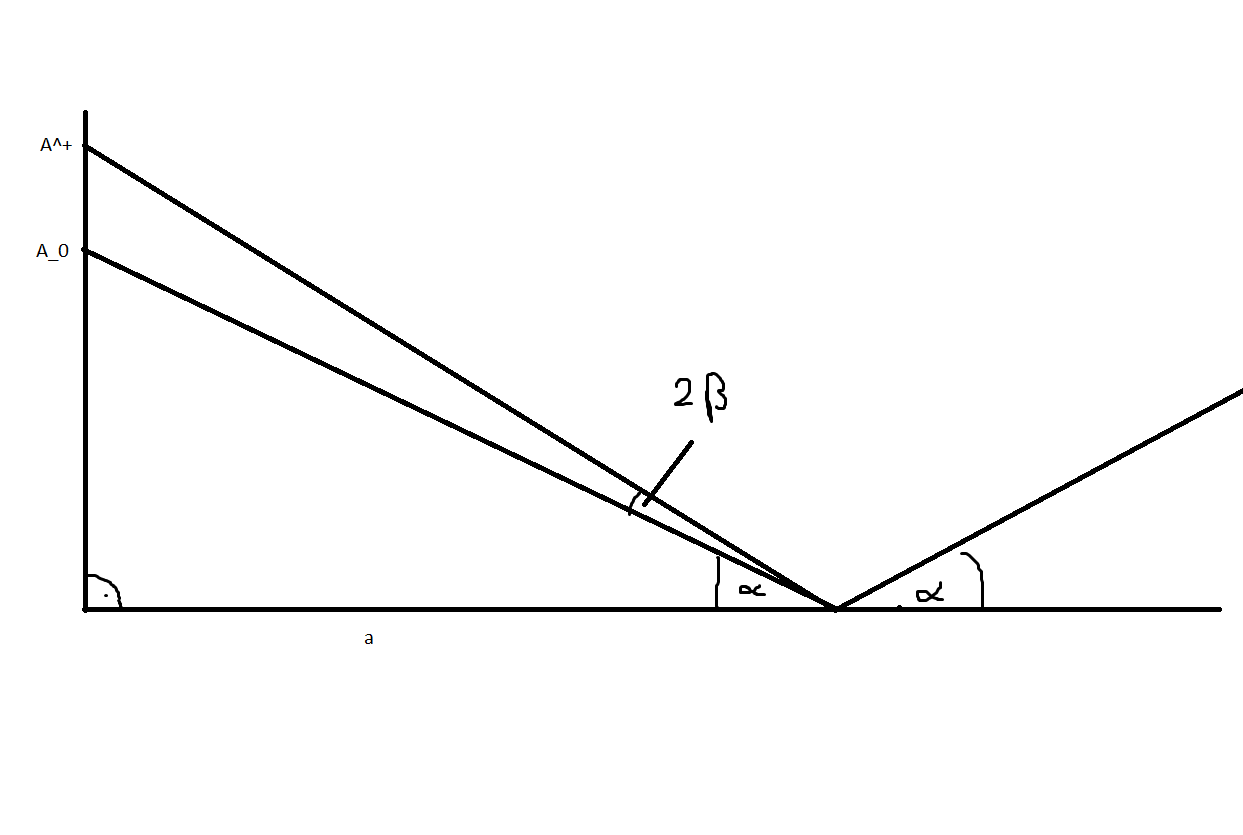
\includegraphics[width=\textwidth]{SkizzeFermi1.png}
			\caption{Aufbau des Demonstrationsversuchs}
			\label{fig:Fermi1}
		\end{figure}
		\begin{figure}
			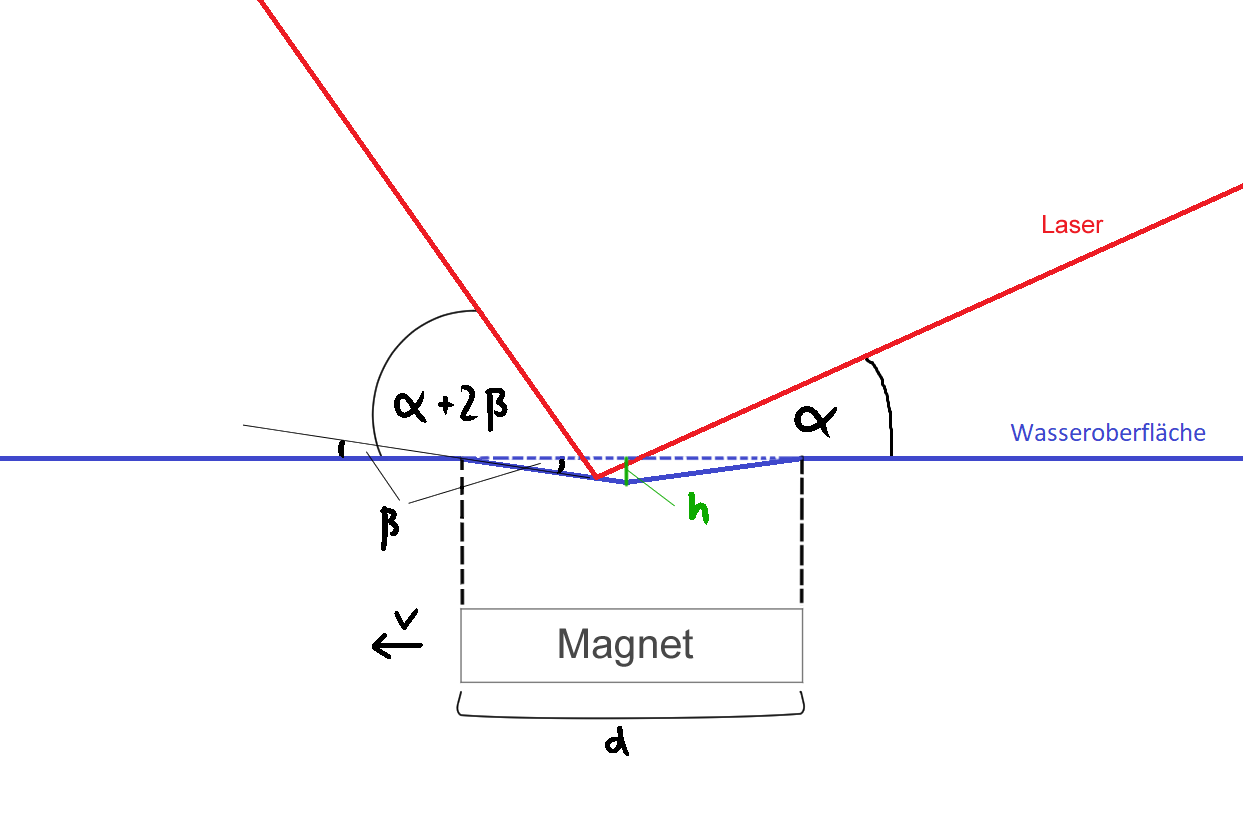
\includegraphics[width=\textwidth]{SkizzeFermi2.png}
			\caption{Genauere Betrachtung der Winkel}
			\label{fig:Fermi2}
		\end{figure}
				
		\subsection*{Fermi-Abschätzung}
				
			Um herauszufinden in welcher Größenordnung die Auslenkung des Wassers liegt, haben wir eine Fermi-Abschätzung durchgeführt.
			Dafür nehmen wir folgende Werte an:
			\begin{equation}
				a = \SI{3,5}{\meter};\quad
				A_0 = \SI{1,2}{\meter};\quad
				\Delta A = \SI{3}{\centi\meter};\quad
				d = \SI{1}{\centi\meter}
			\end{equation}
			Wir erhalten durch Einsetzen in Gleichung \refeq{auslenkung} ein Ergebnis von $h \approx \SI{19}{\micro\meter}$ für die Auslenkung des Wassers, welche in Abb. \ref{fig:zeitverlauf} in Abhängigkeit der Magnetposition\footnote{bzw. der Zeit, bei konstanter Geschwindigkeit des Magneten} ungefähr dargestellt wird. Zudem haben wir den Versuch mit einem Manganchlorid-Hydrat anstelle von Wasser wiederholt und eine deutlich größere Auslenkung, diesmal zunächst in entgegengesetzte Richtung, durch die Reflexion des Lasers wahrgenommen und mit $\Delta A = \SI{0,7}{\meter}$ erhalten wir eine, durch Fermi-Abschätzung der Auslenkung von $h \approx \SI{420}{\micro\meter}$.
			
			\begin{figure}[ht]
				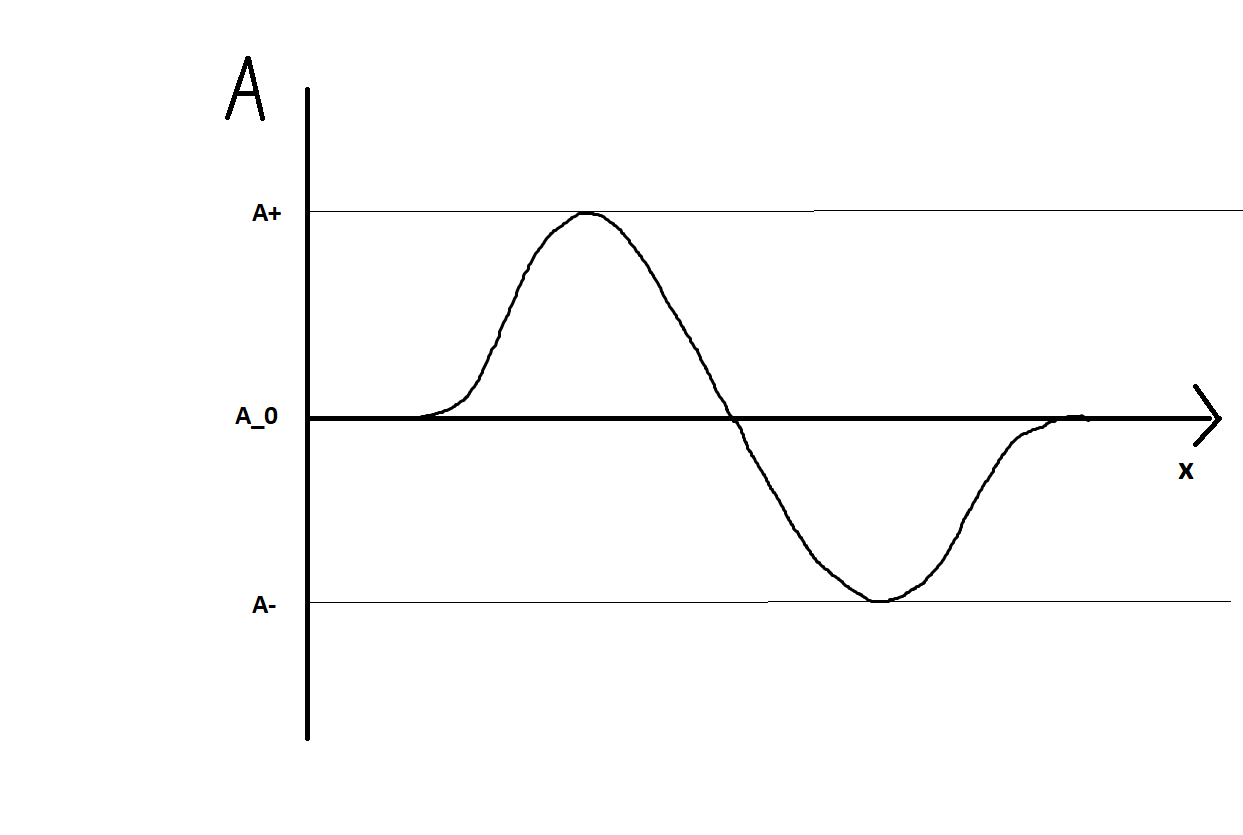
\includegraphics[width=\textwidth]{SkizzeZeitverlaufLichtpunktWasser.png}
				\caption{Verlauf der Position des Lichtpunktes auf dem Schirm gegen die Zeit}
				\label{fig:zeitverlauf}
			\end{figure}

		\subsection*{Schlussfolgerung}
								
			Die von uns ermittelte Größenordnung der Auslenkung für Wasser wirkt realistisch, da es diamagnetisch ist, also nur sehr schwach auf äußere Magnetfelder reagiert sollte, wie von uns ermittelt. Die Betrachtung des Manganchlorids stellt seine paramagnetischen Eigenschaften deutlich in Kontrast zu den Diamagnetischen des Wassers. Diese Kontraste entsprechen den Definitionen von Dia- und Paramagnetismus, da wie wir beobachtet haben (Stärke/Richtung der Auslenkung). 
			
	\section{Versuch 2: Volumensuszeptibilität}		
		
		In dem zweiten Versuch bestimmen wir mit Hilfe der Magnetismuswaage die Volumensuszeptibilität $\chi _V$ von einigen Stoffen. Diese gibt an, wie stark sich ein Stoff magnetisieren lässt.		
		
		\subsection*{Methoden} 
		
			Die Magnetismuswaage, wie sie in Abb. \ref{} dargestellt ist, dient zur Messung der Gewichtsänderung eines Stoffes bei anliegendem äußerem Magnetfeld. Dieses stammt von dem, an dem Schwenkkran angebrachten, Magneten.
			Um eine möglichst genau Messung durchzuführen, bei der die Abstände zwischen Stoffprobe und Magnet gleich sind, verwenden wir eine \SI{1}{\mm} dicke Kunststoffplatte um die Höhe des Schwenkkrans einzustellen.
			
			Damit der Magnet die einfache Messung des Gewichts der Stoffprobe nicht beeinflusst, wird er mit dem Schwenkkran zunächst wegbewegt.
			Für die Messung selber nullen wir zuerst das Gewicht unserer Stoffprobe und fahren dann den Magneten über die Probe.
			
			Die Waage besitzt eine Unsicherheit von \SI{0,001}{\g} und es ergibt sich mit der Unsicherheit der Digitalanzeige eine Gesamtunsicherheit von %TODO
			
			Unsere Stoffproben für diesen Versuch sind Aluminium, pyrolitisches Graphit, Glashalterung (mit und ohne Glas) und eine leere Kunststoffhalterung.
			
			\begin{figure}
				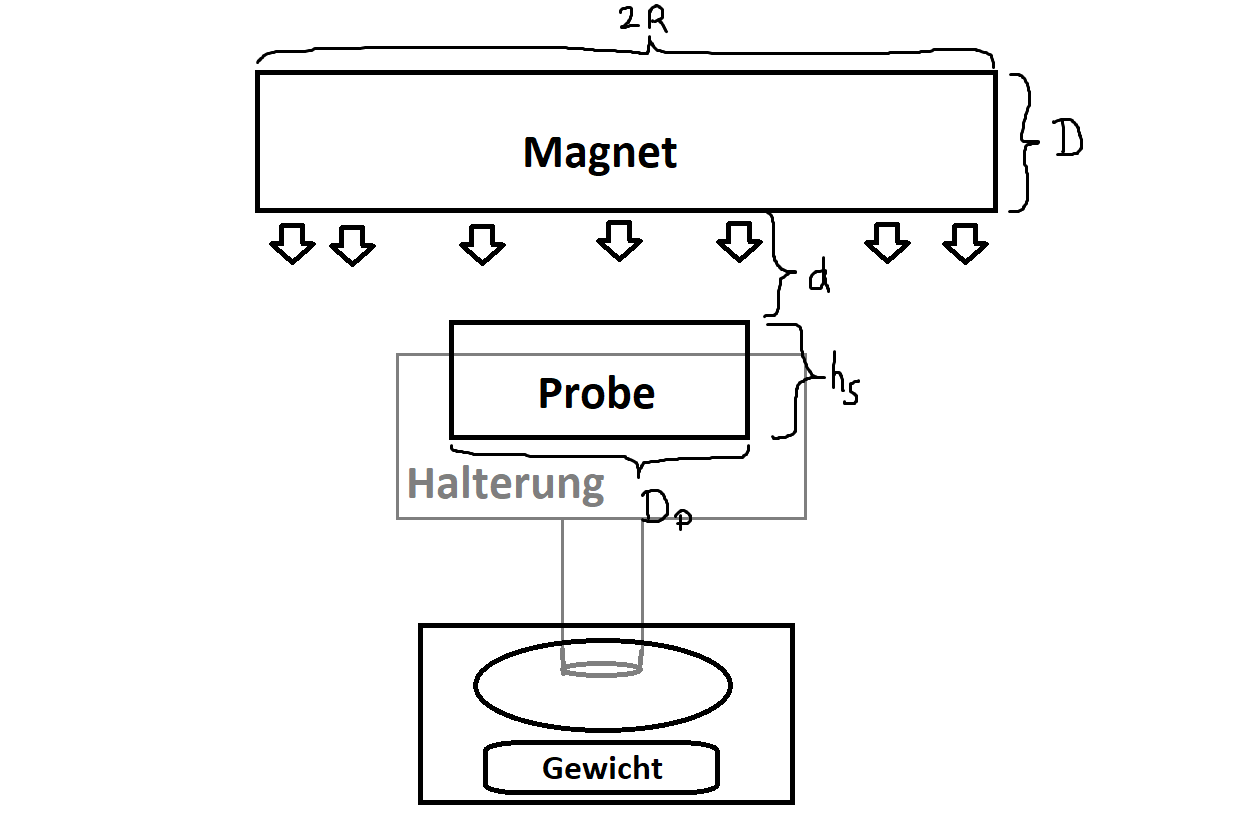
\includegraphics[width=\textwidth]{SkizzeMagnetwaage.png}
				\caption{Aufbau der Magnetismuswaage}
				\label{fig:Magnetismuswaage}
			\end{figure}
		
			Um nun aus dem Gewichtsunterschied die Volumensuszeptibilität $\chi _V$ zu erhalten, gehen wir auf folgende Gleichungen ein:
			\begin{equation*}
				%TODO	
			\end{equation*} 
					
		\subsection*{Messung}
			
			Unsere Messung ergab, durch Anwendung auf die Gleichung \ref{} , die in Tab.\ref{tab:Messergebnisse} dargestellten Ergebnisse für die Volumensuszeptibilitäten $\chi _V$ der Stoffe.
			
				\begin{table}[ht]
				\centering
				\begin{tabular}{l|S|S|S|S|S}
					\hline
					& {Al} & {pyr. Graphit} & {Halterung (Glas)} & {(ohne)} & {Kunststoffhalterung} \\
					\hline
					$\chi _V$ 
					& \SI{0}{\m} %TODO
					& \SI{0}{\m}
					& \SI{0}{\m} 
					& \SI{0}{\m} 
					& \SI{0}{\m} \\
					\hline
				\end{tabular}
				\caption{Ergebnisse der Messungen}
				\label{tab:Messergebnisse}
			\end{table}
					
		\subsection*{Schlussfolgerung}	
			
			Die von uns erhaltenen Wert für die Volumensuszeptibilitäten entsprechen den Erwartungen. Die %TODO
			
			%Glas -> Dia? (Si dia, O2 para) 
			%Al -> Para
			%C -> Dia
		
	\section{Versuch 3: Fallender Neodymmagnet}		
	
		Bei diesem Versuch lassen wir einen Neodymmagneten durch zwei Röhren aus Aluminium fallen. Eine der beiden Röhren besitzt einen Schlitz, der sich über die ganze Länge zieht. Der Aufbau ist in Abb. \ref{fig:Neodymmagnet} dargestellt.
		
		\begin{figure}
			\centering
			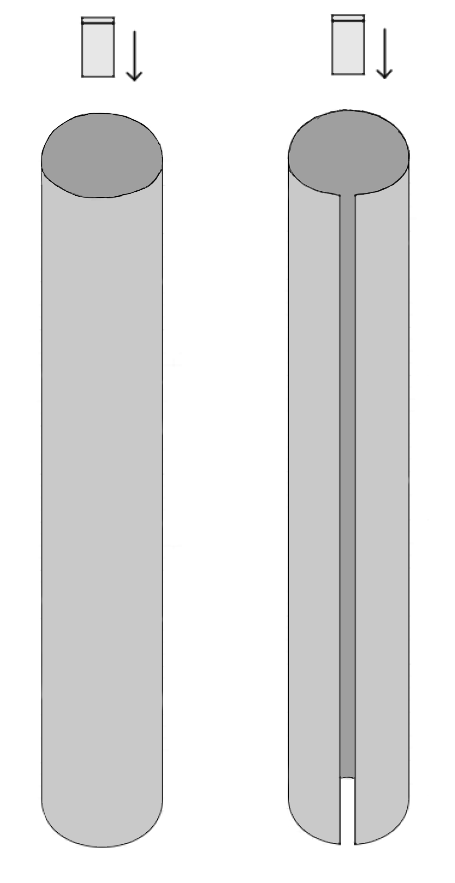
\includegraphics[width=0.4\textwidth]{Neodymmagnet.png}
			\caption{Aufbau des dritten Versuches} %TODO Hier andere Caption?
			\label{fig:Neodymmagnet}
		\end{figure}
		
		\subsection*{Beobachtung}
			
			Wir beobachten, dass der Magnet in den beiden Röhren langsamer fällt als wenn man ihn außerhalb der Röhren fallen lassen würde.
			Hierbei ist jedoch zu beachten, dass der Magnet bei der Röhre mit Schlitz schneller fällt als bei der Anderen.
			
		\subsection*{Schlussfolgerung}	
		
			Das bewegte B-Feld des Magneten induziert einen Kreisstrom in der Aluminiumröhre. Dieser erzeugt dann ein neues B-Feld, welches dem des Magneten entgegenwirkt. Dies führt zu unseren Beobachtungen, dass der Magnet langsamer fällt. %TODO genauer darauf eingehen?
			
			Für die Röhre mit Schlitz wird ebenfalls ein Kreisstrom induziert. Da dieser sich aufgrund der Öffnung jedoch nicht gleichmäßig ausbreiten kann, führt zu einem schwächerem Gegenfeld. Hier fällt der Magnet deswegen ein wenig schneller.		
					
	\section{Versuch 4: Aluminium-Kamm und -Platte} 
	
		Hier haben wir eine Aluminiumplatte und einen -kamm, welche an einer Aufhängung befestigt sind, siehe Abbildung \ref{}. An diesen beiden Objekten bewegen wir nun drei starke aneinander gebundene Magneten von verschiedenen Richtungen und mit unterschiedlichen Geschwindigkeiten.
		Dazu vergleichen wir unsere Beobachtungen für beide Objekte.
		
		\subsection*{Beobachtung}
		
			%TODO
			gleiche Effekte, bei Kamm aber schwächer
			
		\subsection*{Schlussfolgerung}	
		
			%TODO
			Wirbelströme
			%Form von Kamm verhindert Bildung von "größeren" Wirbelströmen -> schwächeres Feld
		
\end{document} 